\ProvidesFile{lecture11.tex}[Лекция 11]


\begin{example}
[V.I.P. пример]
Рассмотрим $p(z) = z^d$ и посмотрим на функцию $p\colon \mathbb C\to \mathbb C$ по правилу $z \mapsto p(z) = z^d$.
Давайте рассмотрим окружность $z(t) = r e^{2\pi i t}$ для $t\in [0, 1]$.
Когда $t$ пробегает от $0$ до $1$, то $z(t) = r e^{2\pi i t}$ пробегает по окружности радиуса $r$ один оборот против часовой стрелки.
Давайте посмотрим на образ этой окружности под действием $p$, получим $p(z(t)) = r^d e^{2\pi i d t}$.
То есть теперь, когда $t$ пробегает от $0$ до $1$ мы пробегаем окружность радиуса $r^d$ но уже $d$ раз против часовой стрелки (делаем $d$ оборотов вместо одного).
% TO DO
% Надо нарисовать картинку!!
\end{example}


\begin{claim}
Пусть $p\in\mathbb C[x]$ -- произвольный не константный многочлен и $z\in \mathbb C$ такая точка, что $p(z)\neq 0$.
Тогда найдется точка $z_1\in \mathbb C$ такая, что $|p(z_1)|<|p(z)|$.
\end{claim}
\begin{proof}

Давайте в начале для отображения $p\colon \mathbb C\to \mathbb C$ сделаем сдвиг координаты в области определения и в области значений вида:
\[
p(u) = p(u + z_0) - p(z_0)
\]
Теперь рассмотрим окружность радиуса $\varepsilon$ вокруг точки $z_0$, то есть $u(t) = \varepsilon e^{2\pi i t}$ при $t\in [0,1]$.
Приблизительный план доказательства следующий.
Я утверждаю, что $p(u(t))$ будет <<приблизительно>> окружность вокруг точки $p(z_0)$ (строгий смысл будет ясен далее).
А раз мы почти окружность, то мы пройдем вокруг точки $p(z_0)$ и где-то уж точно будем ближе к нулю, чем в центре <<почти>> окружности $p(z_0)$.
\begin{center}
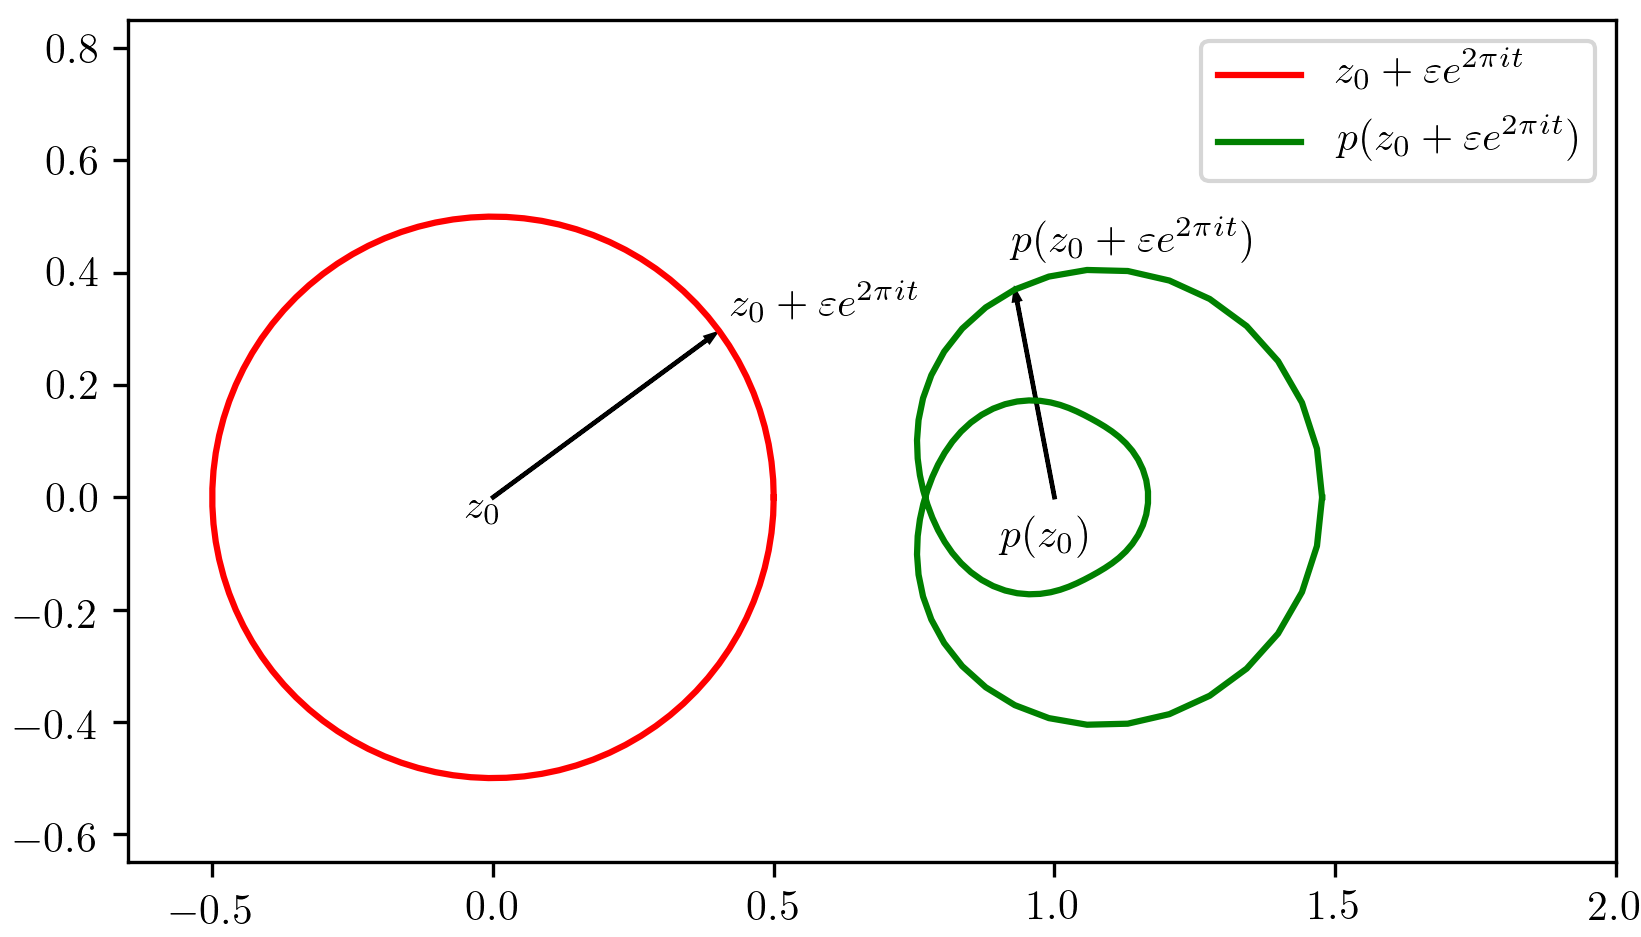
\includegraphics[scale = 0.5]{Figures/graph_cyrcle_cut.png}
\end{center}
Многочлен $p(u)$ в нуле равен нулю, а потому у него нулевой свободный член.
Тогда $p(u) = a_r u^r + \ldots + a_n u^n$, где $a_r$ -- самый младший ненулевой коэффициент ($r > 0$).
Тогда запишем $p(u) = a_r u^r (1 + \omega(u))$, где $\omega(u) = \frac{a_{r+1}}{a_r}u + \ldots + \frac{a_n}{a_r} u^{n-r}$.
Если $|u| < \varepsilon < 1$, то 
\[
|\omega(z)| \leqslant \left| \frac{a_{r+1}}{a_r}u+ \ldots + \frac{a_n}{a_r} u^{n-r}\right| \leqslant  \left|\frac{a_{r+1}}{a_r}\right| \varepsilon+ \ldots + \left|\frac{a_n}{a_r}\right| \varepsilon^{n-r} \leqslant  \left(\left|\frac{a_{r+1}}{a_r}\right|+ \ldots + \left|\frac{a_n}{a_r}\right| \right)\varepsilon
\]
Обозначим последнее выражение за $\delta(\varepsilon)$, оно стремится к нулю при $\varepsilon \to 0$.
Введем следующее обозначение $p_0(u) = a_r u^r$.
Тогда при $\varepsilon < 1$ мы можем оценить значение $p(u(t))$ на окружности $u(t) = \varepsilon e^{2\pi i t}$ следующим образом
\[
|p(u(t)) - p_0(u(t))| \leqslant |a_r| \varepsilon^r \delta(\varepsilon)
\]
Для отображения $p_0(u) = a_r u^r$ найдется $t_0$ такое, что точка $p_0(u(t_0))$ будет ближе к нулю, чем $p(z_0)$ на $ |a_r|\varepsilon^r$.
Но тогда расстояние от $p(u(t_0))$ (по неравенству треугольника) не превосходит
\[
|p(u(t_0))| \leqslant |p_0(u(t_0))| + |p(u(t_0)) - p_0(u(t_0))|  \leqslant |p(z_0)| - |a_r|\varepsilon^r + |a_r|\varepsilon^r\delta(\varepsilon) = |p(z_0)| - |a_r|\varepsilon^r(1 - \delta(\varepsilon))
\]
При малом $\varepsilon$ значение $\delta(\varepsilon)$ будет строго меньше единицы и мы получим точку $z_1 = u(t_0)$, значение в которой будет ближе к нулю, чем значение в $z_0$, что и требовалось.
\end{proof}

\subsection{Многочлены}

В этом разделе я хочу сказать пару слов про многочлены.
Пусть $F$ -- некоторое поле.
Тогда многочлен над полем $F$ -- это картинка вида $f = a_0 + a_1 x + \ldots + a_n x^n$, где $a_i\in F$.
Формально, такая картинка -- это конечная последовательность чисел $(a_0,\ldots,a_n)$, но психологически лучше и правильнее думать именно про картинки.
Еще можно для краткости писать $f = \sum_{k\geqslant 0}a_k x^k$, подразумевая, что в этой сумме только конечное число ненулевых коэффициентов.
Это удобное соображение позволяет удобно записать правила для сложения и умножения многочленов, которые определяются следующим образом
\[
\Bigl( \sum_{k\geqslant 0}a_k x^k\Bigl) + \Bigl( \sum_{k\geqslant 0}b_kx^k\Bigl) =  \sum_{k\geqslant 0}(a_k+b_k) x^k\quad\text{ и }\quad 
\Bigl( \sum_{k\geqslant 0}a_k x^k\Bigl)\Bigl( \sum_{k\geqslant 0}b_k x^k\Bigl) =  \sum_{k\geqslant 0}\Bigl(\sum_{m+n = k} a_m b_n\Bigl) x^k
\]
Таким образом многочлен -- это не функция, а картинка.
Однако, каждый многочлен $f\in F[x]$ задает функцию $F\to F$ по правилу $x\mapsto f(x)$.
Но в случае конечных полей (то есть полей из конечного числа элементов) разные многочлены могут давать одни и те же функции.
Напомню, что степень многочлена $f$ -- это наибольший номер $n$, что коэффициент $a_n\neq 0$.%
\footnote{По-хорошему надо еще аккуратно определить степень нулевого многочлена.
Но ее обычно определяют по ситуации так, как удобнее.
Например можно положить $-1$ или $-\infty$ и есть еще пара способов.
Но об этом можно особенно не запариваться.}

\paragraph{Пример}
\begin{itemize}
\item Пример конечного поля.

Пусть $p\in \mathbb Z$ -- некоторое простое число.
Обозначим через $\mathbb Z_p$ множество остатков по этому числу, то есть $\mathbb Z_p = \{0, 1, \ldots, p-1\}$.
Введем на этом множестве операции сложения и умножения по модулю простого числа $p$, то есть
\[
a + b = a + b\pmod p\quad \text{и}\quad a b = ab \pmod p
\]
Тогда можно проверить, что $Z_p$ является полем, где числа $0$ и $1$ являются нулем и единицей поля.
Единственная аксиома, которая требует усилий -- показать, что любой ненулевой элемент $Z_p$ обратим.
Давайте возьмем произвольный ненулевой элемент $a\in \mathbb Z_p$.
Так как $ a < p$ и $p$ -- простое число, то $(a, p) =1$.
По расширенному алгоритму евклида найдутся целые числа $u, v\in\mathbb Z$ такие, что $1 = u a + vp$.
Рассмотрим это равенство по модулю простого числа $p$ и получим, что
$u a = 1 \pmod p$, а это и означает, что $u$ является обратным к $a$ по умножению.

\item Пример, когда разные многочлены дают одну и ту же функцию.

Рассмотрим многочлены $\mathbb Z_2[x]$.
Тогда $\mathbb Z_2$ состоит только из $0$ и $1$.
В этом случае все многочлены $x^n$ задают одну и ту же функцию.
\end{itemize}

\begin{definition}
 Пусть $F$ -- произвольное поле и $f\in F[x]$ -- некоторый многочлен.
 Если число $a\in F$ является его корнем, то $f$ делится на $x - a$, а значит представляется в виде $f(x) = (x - a) g(x)$ для некоторого $g\in F[x]$.
 Аналогично, если $a$ является корнем $g$, то можно выделить $(x - a)$ и в $g$ и так далее.
 В итоге можно найти разложение $f(x) = (x - a)^k g(x)$, где $g(a) \neq 0$.
 В этом случае говорят, что $k$ -- это кратность корня $a$ в многочлене $f$.
 Корень кратности $1$ называется простым.
\end{definition}


\begin{definition}
Пусть $f\in F[x]$ имеет вид $f = a_0 + a_1 x + \ldots + a_n x^n$.
Определим формальную производную следующим образом $f' = a_1 + 2a_2 x+\ldots + na_n x^{n-1}$ или по-другому $f'=\sum_{k\geqslant 0} k a_k x^{k-1}$.
\end{definition}

Несложно убедиться, что, определив таким образом производную, она удовлетворяет всем естественным свойствам, к которым мы привыкли в анализе.
В качестве упражнения предлагается проверить следующее.

\begin{claim}
Пусть $F$ -- произвольное поле.
Для формальной производной выполнены следующие свойства:
\begin{enumerate}
\item $(f + g)' = f' + g'$ для любых $f,g\in F[x]$.

\item $(\lambda f )' = \lambda f'$ для любых $\lambda\in F$ и $f\in F[x]$.

\item $(fg)' = f' g + fg'$ для любых $f,g\in F[x]$.

\item $f(g(x))' = f'(g(x)) g'(x)$ для любых $f,g\in F[x]$.
\end{enumerate}
\end{claim}


С помощью формальной производной можно проверить кратность корня в произвольном многочлене.
Для начала нам нужно следующее вспомогательное утверждение.

\begin{claim}
Пусть $F$ -- произвольное поле, $f\in F[x]$ -- некоторый многочлен и $a\in F$ -- его корень кратности $k$.
Тогда 
\begin{enumerate}
\item Число $a$ является корнем кратности хотя бы $k-1$ в многочлене $f'$.

\item Если число $k 1 \neq 0$ в $F$, то $a$ является корнем кратности в точности $k - 1$ в многочлене $f'$.
\end{enumerate}
\end{claim}
\begin{proof}
1) По определению имеем $f = (x - a)^k g(x)$ причем $g(a) \neq 0$.
Возьмем производную от $f$, получим
\[
f' = k(x-a)^{k-1}g(x) + (x-a)^k g'(x) = (x-a)^{k-1}(kg(x) + (x-a)g'(x))
\]
и мы видим, что у производной $a$ имеет кратность хотя бы $k-1$.


2) Давайте поймем, когда кратность может вырасти.
Только если множитель $(kg(x) + (x-a)g'(x))$ зануляется в $a$.
Если подставить $a$, то получим $kg(a)$.
Число $g(a)\neq 0$ по выбору, но если $k 1\neq 0$, то и их произведение не ноль в поле $F$, а это будет означать, что кратность корня в точности $k - 1$.
\end{proof}

\paragraph{Примеры и замечания}
\begin{enumerate}
\item
Давайте продемонстрируем ситуацию, когда кратность корня может возрасти.
Например, выберем $F = \mathbb Z_p$ и в качестве многочлена $h$ рассмотрим $x^p - 1$.
Тогда $h' = 0$.
Теперь положим $f = xh(x) = x^{p+1}- x$.
Тогда $f' = h(x) = x^p - 1$.
С другой стороны $x^p - 1 = (x-1)^p$, а значит $1$ имеет кратность $p$ в многочлене $f$.
Но и в многочлене $f'$ $1$ имеет кратность $p$.

\item Если для любого натурального числа $k\in \mathbb N$ в поле $F$ выполнено, $k 1 \neq 0$, то можно следующим образом проверить корень многочлена $f\in F[x]$ на кратность.
Если $a\in F$ -- некоторый корень.
Надо посмотреть на $f'(a)$.
Если это число ноль, то $a$ корень кратности больше $1$, а если не ноль, то кратности в точности $1$.

\item Если $F$ произвольное поле, то общий алгоритм проверки корня на простоту следующий.
Надо взять многочлен $f\in F[x]$, для которого $a$ является корнем.
Посчитать производную $f'$, потом посчитать нод $d(x) = (f, f')$.
Если $d(a) = 0$, то $a$ кратный корень, если $d(a) \neq 0$, то это корень кратности $1$.%
\footnote{Я не буду останавливаться на доказательствах этих фактов.
Все они вам встретятся в курсе алгебры.}
\end{enumerate}



\newpage
\section{Векторные пространства}

\subsection{Идея и определение}

\paragraph{Идея}
Мы с вами до этого изучали много разных объектов, которые не сильно похожи друг на друга.
Например, вектор-столбцы $F^n$, матрицы $\operatorname{M}_{m\,n}(F)$, функции $f\colon X\to F$, многочлены $F[x]$.
Все эти товарищи нам постоянно встречаются и каждый раз приходится для каждого из них все доказывать заново и во время доказательств мы видим, что наши рассуждения повторяются.
Это означает, что на самом деле у всех этих объектов есть некий общий интерфейс, через который мы на самом деле с ним работаем.
Самое главное в этом интерфейсе то, что мы можем брать элементы из этих объектов, умножать эти элементы на числа и складывать между собой.
Абстрактное векторное пространство как раз и формализует идею такого общего интерфейса, через который в множестве можно складывать элементы и умножать на числа.


У такого подхода есть несколько плюсов.
Во-первых, формальное удобство, как только вы что-то сделали для абстрактного векторного пространства и увидели, что что-то конкретное является таковым, то все ваши достижения автоматом применимы в этой конкретной ситуации.
Общий алгоритм для векторного пространства будет одинаково хорошо работать и для столбцов, и для матриц, и для функций и т.д.
Во-вторых, есть менее очевидный бонус.
Когда мы доказываем что-то про абстрактное векторное пространство, то про него надо думать как про $F^n$.
Это поможет вам не потеряться в формализме и догадаться, что откуда берется.
Неформально это означает, что если вы что-то умеет делать для $F^n$, то это автоматически верно для любого векторного пространства!
Формально это не совсем правда, но в классе хороших пространств это так.%
\footnote{Под хорошими тут подразумеваются конечно мерные.}
Тем не менее, даже в классе всех пространств, интуиция из $F^n$ очень полезна.


\paragraph{Определение}
 Следующее определение -- это пример определения с контекстом.
Это означает, что прежде, чем его дать, вы должны зафиксировать некоторую информацию, которая необходима для вашего определения и без это информации оно -- бессмысленный мусор.
У определения векторного пространства в качестве такого контекста выступает некоторое поле $F$.
Это значит, что пока вы не зафиксировали какое-то поле, вы не можете говорить о векторных пространствах над полем $F$, а <<просто векторных пространств>> без указания какого-либо поля не существует.

\begin{definition}\label{def::VectorSpace}
Пусть $F$ -- некоторое фиксированное поле.
Тогда векторное пространство над полем $F$ -- это следующий набор данных $(V, +, \cdot)$, где
\begin{itemize}
\item $V$ -- множество.
Элементы этого множества будут называться векторами.

\item $+\colon V \times V \to V$ -- бинарная операция, то есть правило действующее так $(v,u)\mapsto v + u$, где $u,v \in V$.

\item $\cdot \colon F \times V \to V$ -- бинарная операция , то есть правило действующее так $(\alpha, v)\mapsto \alpha v$, где $\alpha \in F$ и $v\in V$.
\end{itemize}
При этом эти данные удовлетворяют следующим $8$ аксиомам:
\begin{enumerate}
\item {\bf Ассоциативность сложения} Для любых векторов $u,v,w\in V$ верно $(u+v) + w = u + (v+w)$.

\item {\bf Существование нулевого вектора} Существует такой вектор $0\in V$, что для любого $v\in V$ выполнено $0 + v = v + 0 = v$.

\item {\bf Существование противоположного вектора} Для любого вектора $v\in V$ существует вектор $-v\in V$ такой, что $v + (-v) = (-v) + v = 0$.

\item {\bf Коммутативность сложения} Для любых векторов $u,v \in V$ верно $u + v = v + u$.

\item {\bf Согласованность умножения со сложением векторов} Для любого числа $\alpha \in F$ и любых векторов $u,v \in V$ верно $\alpha(v + u) = \alpha v + \alpha u$.

\item {\bf Согласованность умножения со сложением чисел} Для любых чисел $\alpha, \beta\in F$ и любого вектора $v\in V$ верно $(\alpha + \beta)v = \alpha v + \beta v$.

\item {\bf Согласованность умножения с умножением чисел} Для любых чисел $\alpha,\beta\in F$ и любого вектора $v\in V$ верно $(\alpha\beta)v = \alpha(\beta v)$.

\item {\bf Нетривиальность} Для любого $v\in V$ верно $1 v = v$.%
\footnote{Здесь $1\in F$.}
\end{enumerate}
\end{definition}

\paragraph{Примеры}
\begin{enumerate}
\item Поле $F$ (или кто больше привык к вещественным числам $\mathbb R$) является векторным пространством над $F$ (соответственно над $\mathbb R$).

\item Более обще, множество вектор-столбцов $F^n$ является векторным пространством над $F$.

\item Множество матриц $\operatorname{M}_{m\,n}(F)$ является векторным пространством над $F$.

\item Пусть $X$ -- произвольное множество, тогда множество функций $\{f\colon X\to F\}$ является векторным пространством над $F$.
Надо лишь объяснить как складывать функции и умножать на элементы $F$.
Операции поточечные, пусть $f,g\colon X\to F$, тогда функция $(f+g)\colon X\to F$ действует по правилу $(f+g)(x) = f(x) + g(x)$.
Если $\alpha \in F$, то функция $(\alpha f)\colon X\to F$ действует по правилу $(\alpha f)(x) = \alpha f(x)$.

\item Множество многочленов $F[x] = \{a_0+a_1x + \ldots + a_n x^n\mid a_i \in F,\,n\in \mathbb Z_{\geqslant 0}\}$.
Тут надо обратить внимание, что мы подразумеваем под многочленом.
Для нас многочлен -- это НЕ функция, многочлен -- это картинка вида $a_0 + a_1 x + \ldots + a_n x^n$.%
\footnote{Для любителей формализма, можете считать, что многочлен -- это конечная последовательность элементов $F$ вида $(a_0,\ldots,a_n)$, но длина последовательности может быть любой, включая нулевую.}
Складываются и умножаются эти картинки по одинаковым правилам.
Важно, что две такие картинки равны тогда и только тогда, когда у них равные коэффициенты.
Множество всех многочленов $F[x]$ является векторным пространством над $F$.
\end{enumerate}

\paragraph{Замечание}
Стоит отметить, что в обычных векторных пространствах мы привыкли к некоторым свойствам, которые бы хотелось иметь и в общем случае.
Например, в $F^n$ есть единственный нулевой вектор, а аксиомы в общем случае говорят, что нулевой вектор лишь существует.
Однако, можно показать, что нулевой вектора автоматически единственный.
Давайте перечислим некоторые непосредственные следствия из аксиом, которые я оставляю в качестве упражнения:
\begin{enumerate}
\item Нулевой вектор единственный.

\item Для любого $v\in V$ существует единственный $-v$.

\item Для любого вектора $v\in V$ верно $-v = (-1)v$.

\item Для любого вектора $v\in V$ имеем $0 v = 0$.

\item Для любого числа $\alpha \in F$ верно $\alpha 0 = 0$.
\end{enumerate}

\subsection{Подпространство}

Пусть $V$ -- векторное пространство над $F$.
Тогда непустое подмножество $U\subseteq V$ называется подпространством, если на него можно ограничить операции $+$ и $\cdot$ и относительно них оно является векторным пространством.
Давайте определим подпространство формально.
\begin{definition}
Пусть $V$ -- векторное пространство над полем $F$.
Тогда подмножество $U\subseteq V$ называется подпространством, если
\begin{enumerate}
\item $U$ не пусто.%
\footnote{При наличии свойства~(3) это свойство эквивалентно тому, что нулевой вектор $V$ попадает в $U$.
Действительно, если он попадает, то $U$ не пусто.
Наоборот, если $u\in U$ -- какой-то вектор, то $0 = 0 u\in U$ по третьему свойству.}

\item Для любых векторов $u,u'\in U$ верно, что $u+u'\in U$.

\item Для любого скаляра $\alpha\in F$ и вектора $u\in U$ верно, что $\alpha u \in U$.
\end{enumerate}
\end{definition}
Если $U$ -- подпространство в $V$, то на $U$ можно корректно ограничить операции сложения и умножения на скаляр из исходного пространства $V$.
Таким образом у нас получается набор данных $(U, +, \cdot)$ и теперь надо, чтобы выполнялись все аксиомы векторного пространства для них.
Оказывается, что все аксиомы будут выполняться автоматически!
Например, почему у нас будет $0\in U$.
Потому что если мы возьмем любой вектор $u\in U$, то $0 = 0 u \in U$.
Остальное я оставлю в качестве упражнения.

\paragraph{Примеры}
\begin{enumerate}
\item Для любого векторного пространства $V$ подмножества $0$ и $V$ всегда являются подпространствами.

\item Множество $\{y\in F^n \mid Ay = 0\}\subseteq F^n$, где $A\in\operatorname{M}_{m\,n}(F)$, является векторным подпространством в $F^n$.
\end{enumerate}

Обратите внимание, что подпространство из второго примера кажется устроено сложнее, чем векторное пространство, в котором оно лежит $F^n$.
Однако, окажется, что взаимодействие с ними через абстрактный интерфейс векторного пространства происходит абсолютно одинаков.
То есть на самом деле подпространство устроено не сложнее, чем исходное пространство.
Об этом речь пойдет после того, как мы узнаем, что такое базисы и что значит, что какие-то векторные пространства одинаковые.

\subsection{Линейные комбинации}

\paragraph{Мотивация}
Пусть у нас есть векторное пространство $V$ над полем $F$.
Давайте поймем, а что вообще с ним можно делать?
Во-первых, $V$ -- это множество.
Значит из него можно брать элементы.
Во-вторых, там есть операция умножения на числа, то есть любой вектор можно умножить на какое-то число.
В-третьих, у нас вектора можно складывать.
Все это означает, что все что можно делать с векторным пространством, это набрать каких-то векторов из него $v_1,\ldots,v_n$ и написать выражение вида $\alpha_1 v_1 + \ldots + \alpha_n v_n$, для произвольных $\alpha_i\in F$.
Это выражение будет задавать нам какой-то вектор из $V$.
Как мы видим, особенно не разбежишься с разнообразием действий.
Однако, важно, что с помощью подобных выражений можно вытащить абсолютно всю информацию из векторных пространств, которую только возможно.
Именно поэтому все наше внимание будет посвящено выражениям такого вида, так как из них получится узнать все, что только можно про векторные пространства.

\paragraph{Линейные комбинации}

Пусть $V$ -- некоторое векторное пространство над полем $F$ и пусть $v_1,\ldots,v_n\in V$ -- некоторый набор векторов.
Тогда выражение вида $\alpha_1 v_1 +\ldots + \alpha_n v_n$, где $\alpha_i\in F$, называется линейной комбинацией $v_1,\ldots,v_n$.
Линейная комбинация называется тривиальной, если все $\alpha_i = 0$.
В противном случае она называется нетривиальной.

Вектора $v_1,\ldots,v_n\in V$ называются линейно зависимыми, если существует их нетривиальная линейная комбинация равная нулю, то есть для каких-то $\alpha_i\in F$ (так что хотя бы один не равен нулю) выражение $\alpha_1 v_1+\ldots + \alpha_n v_n = 0$.
Подчеркнем, что вектора линейно независимы, если из равенство $\alpha_1 v_1 + \ldots + \alpha_n v_n = 0$ следует, что все $\alpha_i = 0$.

\paragraph{Примеры}
\begin{enumerate}
\item Вектор $0$ всегда линейно зависим.

\item Вектор $v\in V$ линейно зависим тогда и только тогда, когда он равен нулю.

\item Вектора $v_1, v_2 \in V$ линейно зависимы тогда и только тогда, когда они пропорциональны (то есть один из них равен другому умноженному на элемент поля).
\end{enumerate}

\paragraph{Линейная оболочка}

Пусть $E\subseteq V$ -- некоторое подмножество в векторном пространстве $V$ над полем $F$.
Тогда обозначим через $\langle E \rangle$ множество всех линейных комбинаций векторов из $E$, то есть
\[
\langle E \rangle = \{\alpha_1 v_1 + \ldots + \alpha_n v_n \mid \alpha_i\in F,\, v_i \in E,\, n\in\mathbb N\}
\]
Сделаем важное замечание, если $E = \varnothing$ пусто, то $\langle \varnothing \rangle$ полагаем равным нулевому подпространству (подпространству состоящему только из нуля).
Это полезное и удобное соглашение можно понимать так: если берется линейная комбинация с нулевым числом слагаемых, то она равна нулю.

Заметим, что $\langle E \rangle$ является наименьшим векторным подпространством содержащим $E$.
Потому, для любого подпространства $U\subseteq V$ верно $\langle U \rangle  = U$.


\paragraph{Пример}

Полезно держать перед глазами следующий пример.
Пусть $V = \mathbb R^3$ -- пространство, $e_1 =(1,0,0)$, $e_2 = (0,1,0)$, $e_3 = (0,0,1)$ три вектора вдоль координатных осей.
Тогда $\langle e_1\rangle$, $\langle e_2\rangle$ и $\langle e_3\rangle$ -- это в точности координатные оси.
Подпространства $\langle e_1, e_2\rangle$, $\langle e_1, e_3\rangle$ и $\langle e_2, e_3\rangle$ -- это плоскости содержащие пары координатных осей, $\langle e_1, e_2, e_3\rangle$ будет совпадать со всем пространством $\mathbb R^3$.

